% =====================================================================
%  TKCE — End-to-end pipeline diagram with a worked example
%  Compiles standalone:  pdflatex pipeline_diagram.tex
%  To reuse in the paper: copy the tikzpicture (and the \tikzset styles).
% =====================================================================
\documentclass[11pt]{article}
\usepackage[margin=0.9in]{geometry}
\usepackage{amsmath,amssymb}
\usepackage{booktabs}
\usepackage{array}
\usepackage{tikz}
\usetikzlibrary{arrows.meta, positioning, fit, backgrounds, calc}
\newcommand{\R}{\mathbb{R}}
\newcommand{\ind}{\mathbf{1}}
\newcommand{\code}[1]{\texttt{#1}}

\tikzset{
  data/.style={rounded corners=4pt, draw=blue!55, fill=blue!8, text width=6.1cm,
               align=center, inner sep=5pt, font=\small},
  proc/.style={draw=orange!75, fill=orange!13, text width=6.1cm,
               align=center, inner sep=5pt, font=\small, thick},
  ex/.style={rounded corners=2pt, draw=gray!45, fill=gray!7, text width=5.6cm,
             align=left, font=\scriptsize, inner sep=4pt},
  arr/.style={-{Stealth[length=2.6mm]}, thick, draw=black!65},
  lnk/.style={dashed, draw=gray!55, shorten >=1pt},
}

\begin{document}
\begin{center}
{\Large\textbf{TKCE: end-to-end pipeline}}\\[2pt]
{\small Worked example: \code{eye\_movements} --- 7{,}608 rows, 20 numerical
features, binary balanced target}
\end{center}
\vspace{-2mm}

% =====================================================================
\section*{1. The flow (left: what happens \quad right: the example)}
% =====================================================================
\begin{center}
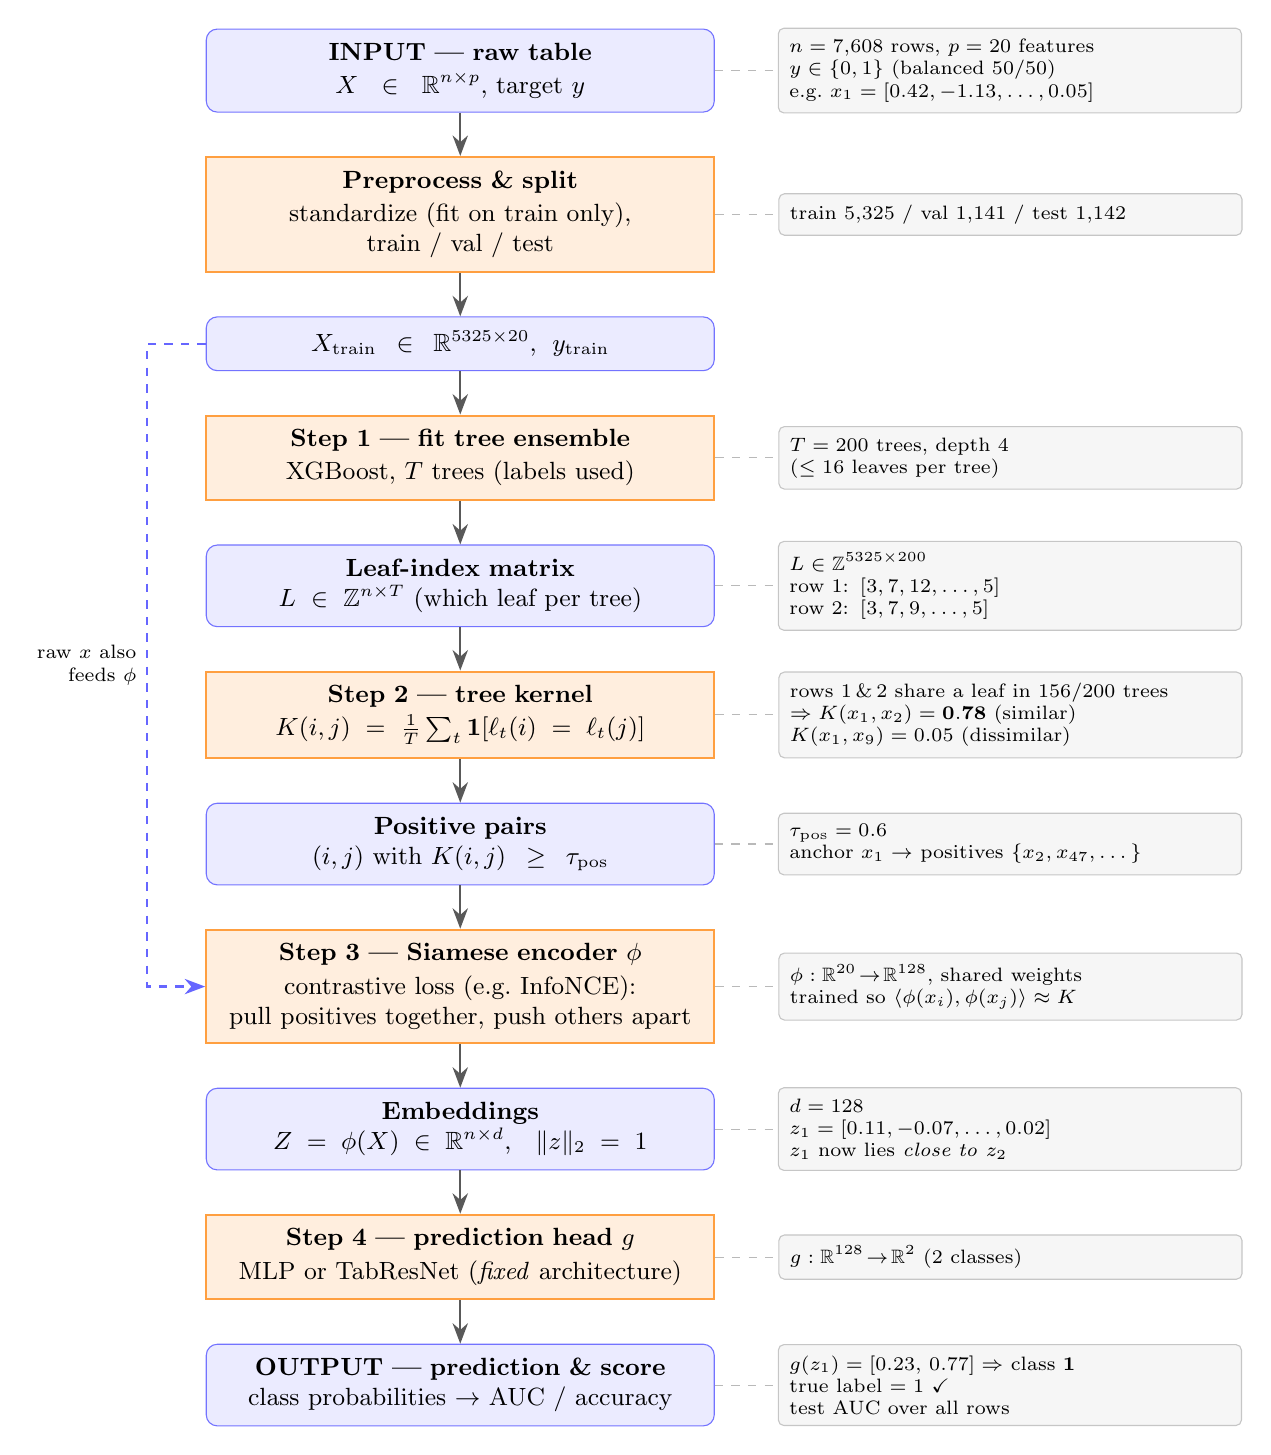
\begin{tikzpicture}[node distance=5.5mm]

\node[data] (raw)
  {\textbf{INPUT --- raw table}\\[1pt]
   $X\in\R^{n\times p}$, target $y$};
\node[ex, right=8mm of raw] (exraw)
  {$n=7{,}608$ rows, $p=20$ features\\
   $y\in\{0,1\}$ (balanced 50/50)\\
   e.g.\ $x_1=[0.42,-1.13,\dots,0.05]$};

\node[proc, below=of raw] (prep)
  {\textbf{Preprocess \& split}\\[1pt]
   standardize (fit on train only), \\ train / val / test};
\node[ex, right=8mm of prep] (exprep)
  {train $5{,}325$ / val $1{,}141$ / test $1{,}142$};

\node[data, below=of prep] (xtr)
  {$X_{\text{train}}\in\R^{5325\times 20}$,\; $y_{\text{train}}$};

\node[proc, below=of xtr] (trees)
  {\textbf{Step 1 --- fit tree ensemble}\\[1pt]
   XGBoost, $T$ trees (labels used)};
\node[ex, right=8mm of trees] (extrees)
  {$T=200$ trees, depth 4\\ ($\le 16$ leaves per tree)};

\node[data, below=of trees] (leaves)
  {\textbf{Leaf-index matrix}\\ $L\in\mathbb{Z}^{n\times T}$ (which leaf per tree)};
\node[ex, right=8mm of leaves] (exleaves)
  {$L\in\mathbb{Z}^{5325\times200}$\\
   row 1: $[3,7,12,\dots,5]$\\
   row 2: $[3,7,9,\dots,5]$};

\node[proc, below=of leaves] (kernel)
  {\textbf{Step 2 --- tree kernel}\\[1pt]
   $K(i,j)=\frac{1}{T}\sum_{t}\ind[\ell_t(i)=\ell_t(j)]$};
\node[ex, right=8mm of kernel] (exkernel)
  {rows 1\,\&\,2 share a leaf in 156/200 trees\\
   $\Rightarrow K(x_1,x_2)=\mathbf{0.78}$ (similar)\\
   $K(x_1,x_9)=0.05$ (dissimilar)};

\node[data, below=of kernel] (pairs)
  {\textbf{Positive pairs}\\ $(i,j)$ with $K(i,j)\ge\tau_{\text{pos}}$};
\node[ex, right=8mm of pairs] (expairs)
  {$\tau_{\text{pos}}=0.6$\\
   anchor $x_1 \to$ positives $\{x_2,x_{47},\dots\}$};

\node[proc, below=of pairs] (enc)
  {\textbf{Step 3 --- Siamese encoder $\phi$}\\[1pt]
   contrastive loss (e.g.\ InfoNCE):\\
   pull positives together, push others apart};
\node[ex, right=8mm of enc] (exenc)
  {$\phi:\R^{20}\!\to\!\R^{128}$, shared weights\\
   trained so $\langle\phi(x_i),\phi(x_j)\rangle\approx K$};

\node[data, below=of enc] (emb)
  {\textbf{Embeddings}\\ $Z=\phi(X)\in\R^{n\times d}$, \; $\|z\|_2=1$};
\node[ex, right=8mm of emb] (exemb)
  {$d=128$\\
   $z_1=[0.11,-0.07,\dots,0.02]$\\
   $z_1$ now lies \emph{close to} $z_2$};

\node[proc, below=of emb] (head)
  {\textbf{Step 4 --- prediction head $g$}\\[1pt]
   MLP or TabResNet (\emph{fixed} architecture)};
\node[ex, right=8mm of head] (exhead)
  {$g:\R^{128}\!\to\!\R^{2}$ (2 classes)};

\node[data, below=of head] (out)
  {\textbf{OUTPUT --- prediction \& score}\\
   class probabilities $\to$ AUC / accuracy};
\node[ex, right=8mm of out] (exout)
  {$g(z_1)=[0.23,\,0.77]\Rightarrow$ class \textbf{1}\\
   true label $=1$ \checkmark\\
   test AUC over all rows};

\foreach \a/\b in {raw/prep, prep/xtr, xtr/trees, trees/leaves, leaves/kernel,
                   kernel/pairs, pairs/enc, enc/emb, emb/head, head/out}
  \draw[arr] (\a) -- (\b);

\foreach \a/\b in {raw/exraw, prep/exprep, trees/extrees, leaves/exleaves,
                   kernel/exkernel, pairs/expairs, enc/exenc, emb/exemb,
                   head/exhead, out/exout}
  \draw[lnk] (\a) -- (\b);

% the raw features are ALSO the encoder's input (not just the leaves)
\draw[arr, dashed, draw=blue!60]
  (xtr.west) -- ++(-0.75,0) |- node[pos=0.25, left, font=\scriptsize, align=right]
  {raw $x$ also\\feeds $\phi$} (enc.west);

\end{tikzpicture}
\end{center}

\noindent\textbf{Note.} The trees are used \emph{only} to define \emph{which rows
are similar} (the kernel). The encoder $\phi$ still reads the \emph{raw} feature
vector $x$ --- that is why the finished model can embed a brand-new row at test
time without re-running the trees.

\newpage
% =====================================================================
\section*{2. Input / output of every stage}
% =====================================================================
\begin{center}\small
\begin{tabular}{@{}p{3.0cm} p{4.5cm} p{4.5cm}@{}}
\toprule
\textbf{Stage} & \textbf{Input} & \textbf{Output} \\
\midrule
Preprocess \& split & raw table $7608\times20$, $y$ &
  $X_{\text{train}} 5325\times20$, val, test \\
\addlinespace
1. Tree ensemble & $X_{\text{train}}$, $y_{\text{train}}$ &
  fitted forest ($T=200$ trees) \\
\addlinespace
\phantom{1.} leaf lookup & $X$ (any split) &
  leaf-index matrix $L$: $n\times200$ integers \\
\addlinespace
2. Tree kernel & two rows' leaf vectors &
  similarity $K(i,j)\in[0,1]$ \\
\addlinespace
3. Pair mining & $K$, threshold $\tau_{\text{pos}}$ &
  list of (anchor, positive) pairs \\
\addlinespace
4. Encoder $\phi$ (train) & raw $x$ + the pairs &
  trained encoder $\phi:\R^{20}\!\to\!\R^{128}$ \\
\addlinespace
\phantom{4.} encoder (apply) & one row $x\in\R^{20}$ &
  embedding $z\in\R^{128}$, $\|z\|_2=1$ \\
\addlinespace
5. Head $g$ & embedding $z\in\R^{128}$ &
  class probabilities $\in\R^{2}$ \\
\addlinespace
6. Evaluation & probabilities + true $y$ &
  AUC, accuracy \\
\bottomrule
\end{tabular}
\end{center}

% =====================================================================
\section*{3. The two ways to train stages 3--5}
% =====================================================================
\begin{center}
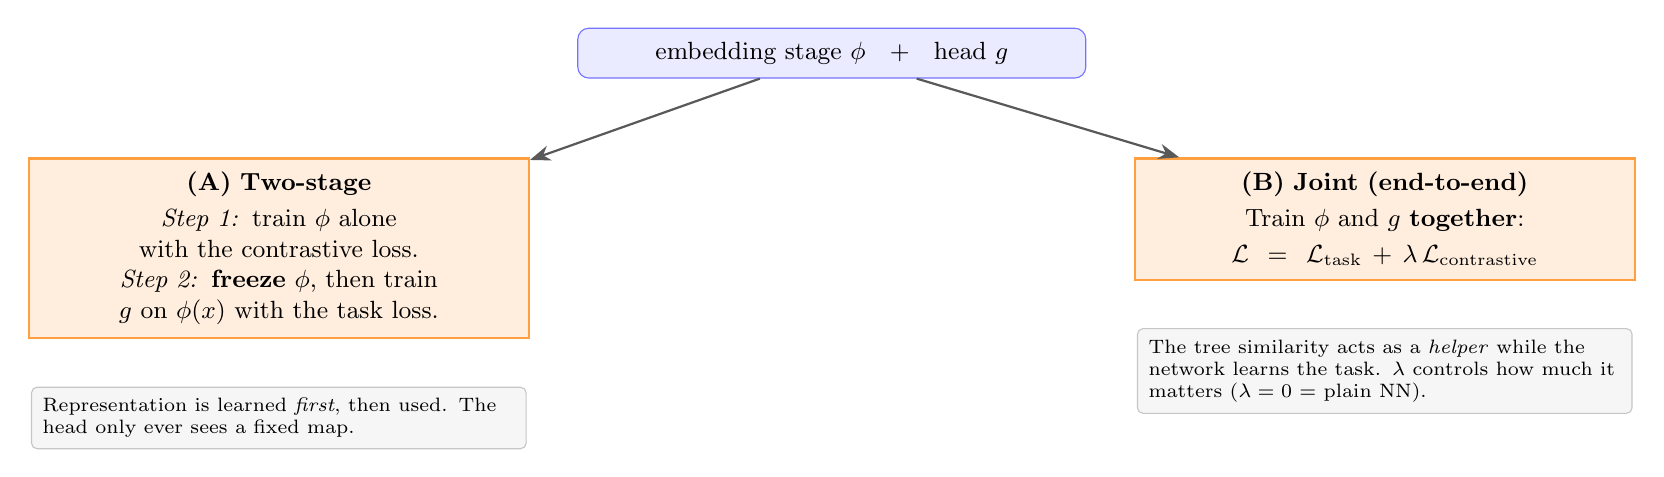
\begin{tikzpicture}[node distance=6mm]
\node[data] (z) {embedding stage $\phi$ \; + \; head $g$};

\node[proc, below left=10mm and 6mm of z, text width=6.0cm] (two)
  {\textbf{(A) Two-stage}\\[2pt]
   \emph{Step 1:} train $\phi$ alone with the contrastive loss.\\
   \emph{Step 2:} \textbf{freeze} $\phi$, then train $g$ on $\phi(x)$ with the
   task loss.};
\node[proc, below right=10mm and 6mm of z, text width=6.0cm] (joint)
  {\textbf{(B) Joint (end-to-end)}\\[2pt]
   Train $\phi$ and $g$ \textbf{together}:\\[2pt]
   $\mathcal{L}=\mathcal{L}_{\text{task}}
    +\lambda\,\mathcal{L}_{\text{contrastive}}$};

\node[ex, below=6mm of two, text width=6.0cm]
  {Representation is learned \emph{first}, then used. The head only ever sees a
   fixed map.};
\node[ex, below=6mm of joint, text width=6.0cm]
  {The tree similarity acts as a \emph{helper} while the network learns the task.
   $\lambda$ controls how much it matters ($\lambda=0$ = plain NN).};

\draw[arr] (z) -- (two);
\draw[arr] (z) -- (joint);
\end{tikzpicture}
\end{center}

\vspace{2mm}
\noindent\textbf{In one sentence:} the trees say \emph{which rows are alike};
the contrastive encoder turns that into \emph{coordinates where alike rows sit
close}; and an ordinary neural head makes the prediction from those coordinates.

\end{document}
